\documentclass[aspectratio=1610,xcolor=dvipsnames]{beamer}
\usepackage{theme}
\usepackage[utf8x]{inputenc}

\usepackage[english]{babel}
\usepackage{calligra}
\usepackage{subcaption}
\usepackage{hyperref}

% Graphics and video
\usepackage{graphicx,float,wrapfig}
\usepackage{animate}
% \usepackage{media9}
% \usepackage{multimedia}
\graphicspath{
  {../assets/}%
}
% \addmediapath{
%     ../assets/
% }


% args: big, bigg, Big, Bigg
\newcommand{\parenth}[2][]{#1(#2#1)}
\renewcommand{\bold}[1]{\textbf{\structure{#1}}}


  
\author[Conti \and Daniotti]{Samuele Conti \and Filippo Daniotti}
\title[Global Motion Estimation]{\textsc{Global Motion Estimation}}
\subtitle{An indirect, multiscale and robust approach}
\institute[DISI - University of Trento]{Department of Information Engineering\\and Computer Science}
\date{April 20, 2022}


\AtBeginSection[]
{
    \begin{frame}
        \frametitle{Table of Contents}
        \tableofcontents[currentsection]
    \end{frame}
}

\begin{document}

\begin{frame}
    \titlepage
    \begin{figure}[H]
        \begin{center}
            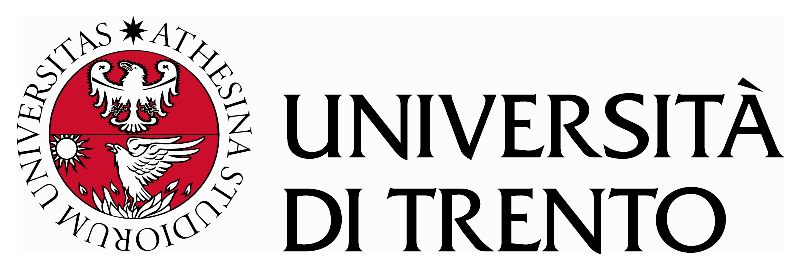
\includegraphics[width=0.4\linewidth]{marchio_unitrento_colore_it_202002.eps}
        \end{center}
    \end{figure}
\end{frame}

\begin{frame}
    \tableofcontents[sectionstyle=show,subsectionstyle=show/shaded/hide,subsubsectionstyle=show/shaded/hide]
\end{frame}

\section{Introduction}
\begin{frame}{Introduction}
    In this work we are going to present:
    \begin{itemize}
        \item a broad introduction to the problem of global motion estimation
        \item an overview of the theoretical foundations of our solution
        \item the framework we developed from the aforementioed literature
        \item an analysis of the performances of our solution 
        \item a brief discussion of the limitations and possible improvements
    \end{itemize}
\end{frame}

\section{The problem}
\begin{frame}{Global motion estimation}
    The motion in videos can be analized as the displacement of pixel per pair of frames
    \bigskip

    \begin{columns}
        \begin{column}{0.45\textwidth}
            Is usually the combination of two different motions:
            \begin{itemize}
                \item the actual motion of objects in the scene
                \item the egomotion of the camera
            \end{itemize}
        \end{column}
        \begin{column}{0.45\textwidth}
            \begin{figure}[H]
                \animategraphics[loop,autoplay,width=.6\linewidth]{20}{gifs/pan240/pan240-}{0}{40}
                \caption{Local motion vs. egomotion}
            \end{figure}
        \end{column}
    \end{columns}

    \begin{alertblock}{The problem}
        Global motion estimation aims to extract the camera global motion patterns in a video
    \end{alertblock}
\end{frame}

\begin{frame}{Motion models}
    Motion models describe camera motion patterns through equations
    \bigskip
    \begin{columns}
        \begin{column}{0.35\textwidth}
            \begin{figure}
                \centering
                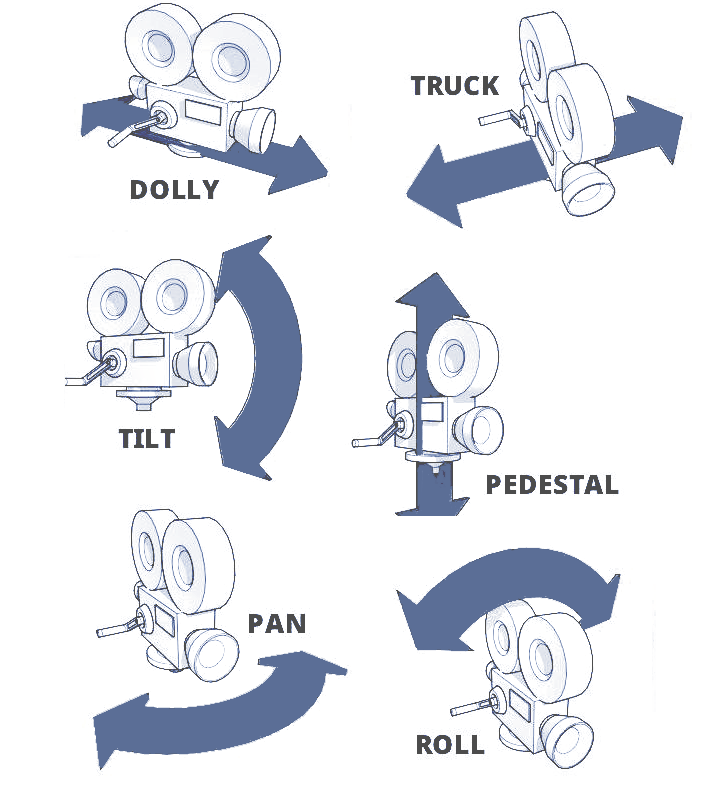
\includegraphics[width=.7\linewidth]{../assets/images/camera-movement.png}
                \caption{Different models describe different types of camera motion}
                \label{fig:camera-motion}
            \end{figure}
        \end{column}
        \begin{column}{0.65\textwidth}
            The displacement of a pixel across frames as a function of some parameters
            \begin{equation}
    \label{eq:affine-model-representation}
    p' = 
    \begin{bmatrix}
        X' \\ Y' \\ Z'
    \end{bmatrix}
    =
    \begin{bmatrix}
        r_1 & r_2 & r_3 \\
        r_4 & r_5 & r_6 \\
        r_7 & r_8 & r_9 
    \end{bmatrix}
    \begin{bmatrix}
        X \\ Y \\ Z
    \end{bmatrix}
    +
    \begin{bmatrix}
        T_X \\ T_Y \\ T_Z
    \end{bmatrix}
    = Rp + T
\end{equation}
            E.g. for the \bold{affine model} (our choice) parameter vecotr is \(a = [a_0, a_1, a_2, b_0, b_1, b_2]\)
        \end{column}
    \end{columns}
\end{frame}

% \section{Theory}
% \begin{frame}{Dealing with GME}
%     Most of the existing algorithms that deal with global motion estimation assume that camera motion can be described as a  \bold{parameterized motion model}.
%     \begin{block}{Parameterized motion model}
%         An equation that describes the expected shape of the motion vector for each still pixel, given a certain movement of the camera
%     \end{block}
%     \bigskip
%     Different global motion patterns (translation, rotation, panning, et cetera) are described by different models
%     \begin{exampleblock}{Some well-known global motion models}
%         \begin{itemize}
%             \item translation model
%             \item affine model
%             \item projective model
%         \end{itemize}
%     \end{exampleblock}
% \end{frame}

\begin{frame}{Estimating parameters}
    There are two main approaches, both of which aim to minimize a prediction error
    \bigskip
    \begin{itemize}
        \item \bold{direct methods} work in the pixel domain
        \item \bold{indirect methods} work with motion fields
    \end{itemize}
    \bigskip
    For our solution we opted for \bold{indirect methods}
    \begin{block}{Indirect paramter update}
        The parameter vector \(a\) is updated by choosing the parameters that minimize the dissimilarity of the \(gt(x)\) and the prediction \(MM(x,a)\) for a point \(x\)
        \begin{equation}
    \label{eq:indirect-estimation}
    a = \arg \min_a \sum_p E(gt(p) - MM(p, a))
\end{equation}
    \end{block}
\end{frame}

% \begin{frame}{Indirect parameter estimation}
    % \begin{block}{Fitting error}
    %     Compare ground truth \(d(x)\) to the estimate with current params \(d(x;a)\)
    %     % Given a motion field \(d(x)\) computed at a set of sufficiently dense points \(x \in \Lambda ' \subset \Lambda \) and the motion field \(d(x;a)\) given by the model w/ current parameters \(a\), we compute the fitting error as
    %     \begin{equation}
    %         \label{eq:fitting-error}
    %         E = \sum_{x \in \Lambda '} | d(x;a) - d(x) |^p
    %     \end{equation}

    % \end{block}

    % Global motion can be approximed as a polynomial function, so \(d(x;a)\) is a linear function of \(a\) \(\to\) \(d(x;a) = [A(x)]a\)
    % % \bigskip
    
    % \begin{block}{Minimizing the error}
    %     Assuming \(p = 2\) we can recompute \(a\) minimizing \(E\) as follows
    
    %     \begin{equation}
    %         \label{eq:min-fit-err}
    %         \frac{\partial E}{\partial a} = 0 
    %         \quad
    %         \Rightarrow 
    %         \quad
    %         a = \parenth[\Bigg]{\sum_{x \in \Lambda '} [A(x)]^T[A(x)]}^{-1}\parenth[\Bigg]{\sum_{x \in \Lambda '} [A(x)]d(x)}
    %     \end{equation}    
    % \end{block}
% \end{frame}

\section{Implementation}
\begin{frame}{Overview}
    \begin{columns}
        \begin{column}{0.45\textwidth}
            \begin{figure}[H]
                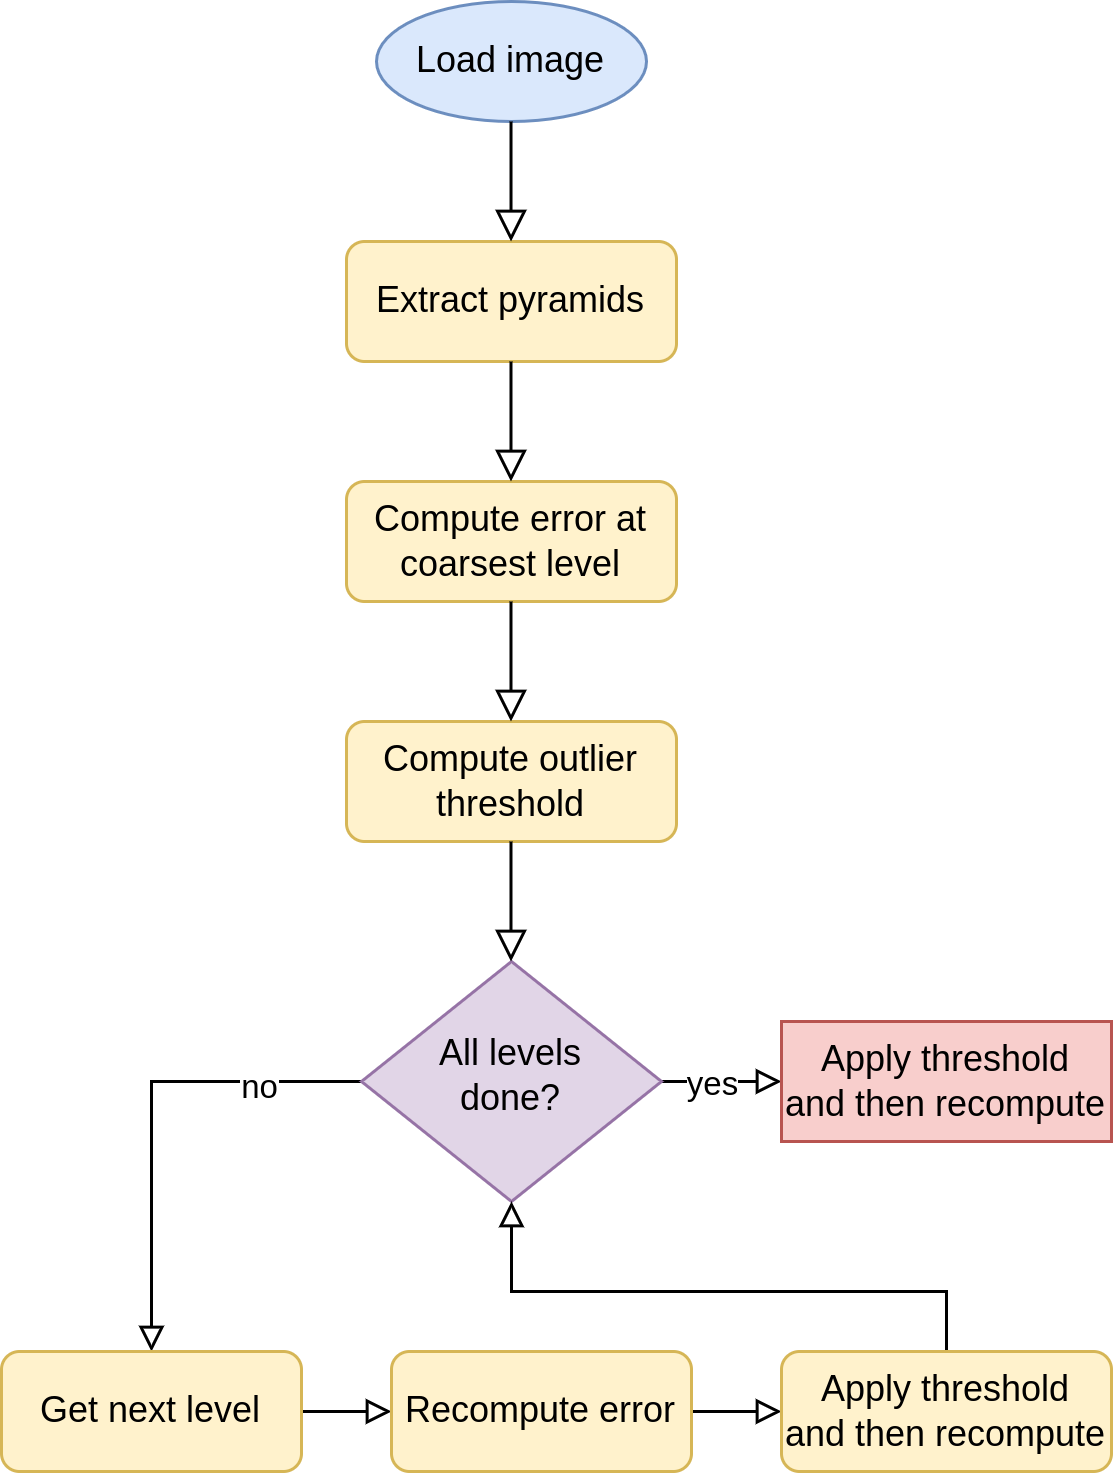
\includegraphics[keepaspectratio,width=.8\textwidth]{images/implementation-flow.png}
                \caption{Flowchart of our framework}
            \end{figure}
        \end{column}
        \begin{column}{0.45\textwidth}
            Implementation choices:
            \begin{itemize}
                \item Affine model
                \item Indirect method
                \item Block-based motion estimation
                \item Multiscale
                \item Robust
            \end{itemize}
        \end{column}
    \end{columns}
\end{frame}

\subsection{Motion estimation}
\begin{frame}{Block-based motion estimation}
	The affine model requires a dense motion field when computing the parameters, which we compute via a block-based approach

	\bigskip	
	We started with 3 well-established BBME algorithms:
	\begin{itemize}
		\item exhaustive search
		\item three-step search
		\item 2D log search
	\end{itemize}
    Then, we search for new algorithms in the literature and landed on \bold{diamond search}
	\bigskip
    \begin{block}{Displaced frame difference}
        As DFD, we tried both 1-norm (MAE) and 2-norm (MSE)        
    \end{block}
    
\end{frame}

\begin{frame}{Exhaustive search}
	\begin{figure}
		\begin{minipage}{.45\textwidth}
            \centering
            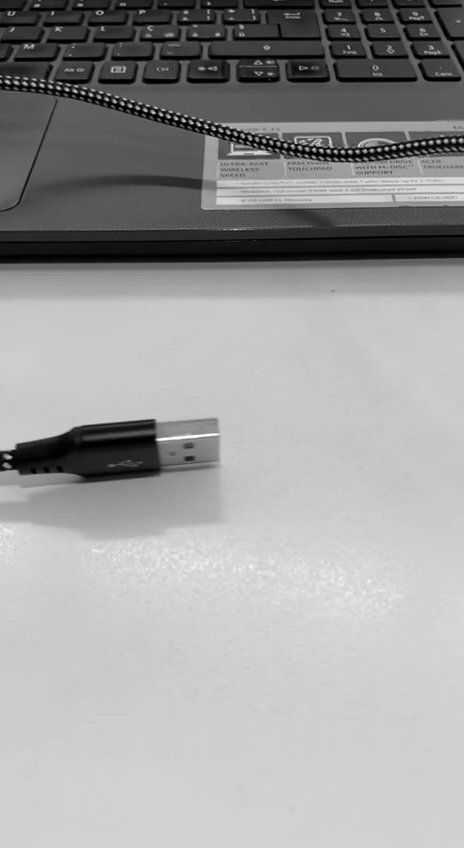
\includegraphics[keepaspectratio, width=.55\linewidth]{images/bbme-im.png}
            \subcaption{Target frame}
            \label{fig:bbme-0-im}
		\end{minipage}
		\begin{minipage}{.45\textwidth}
            \centering
            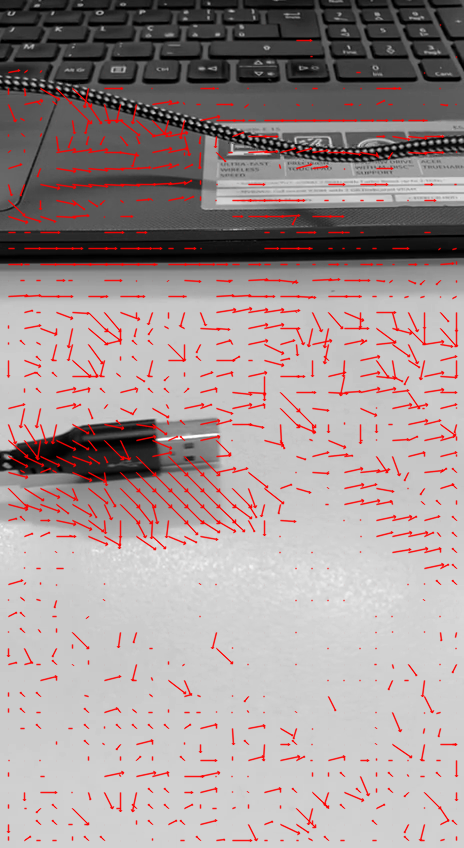
\includegraphics[keepaspectratio, width=.55\linewidth]{images/bbme-0-res.png}
            \subcaption{Needle diagram}
            \label{fig:bbme-0-res}
		\end{minipage}
        \label{fig:bbme-0}
        \caption{Motion field result of our EBBME implementation}
	\end{figure}
\end{frame}

\begin{frame}{Three-step search}
	\begin{figure}[H]
		\begin{minipage}{.45\textwidth}
            \centering
            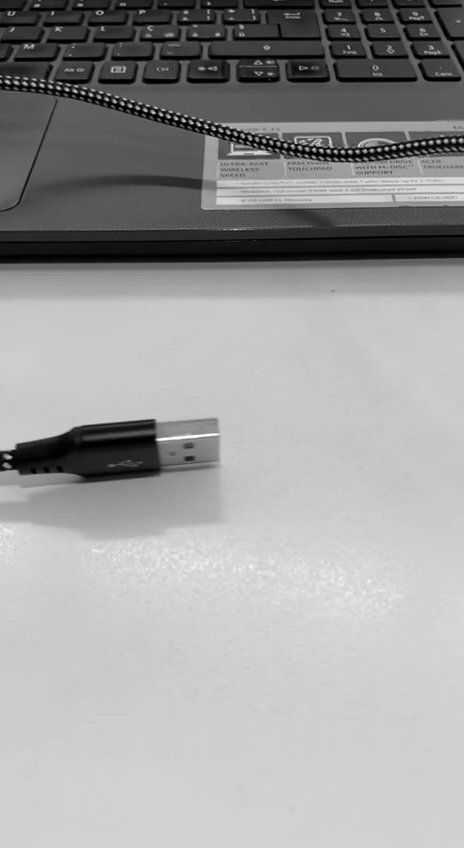
\includegraphics[keepaspectratio, width=.55\linewidth]{images/bbme-im.png}
            \subcaption{Target frame}
            \label{fig:bbme-1-im}
		\end{minipage}
		\begin{minipage}{.45\textwidth}
            \centering
            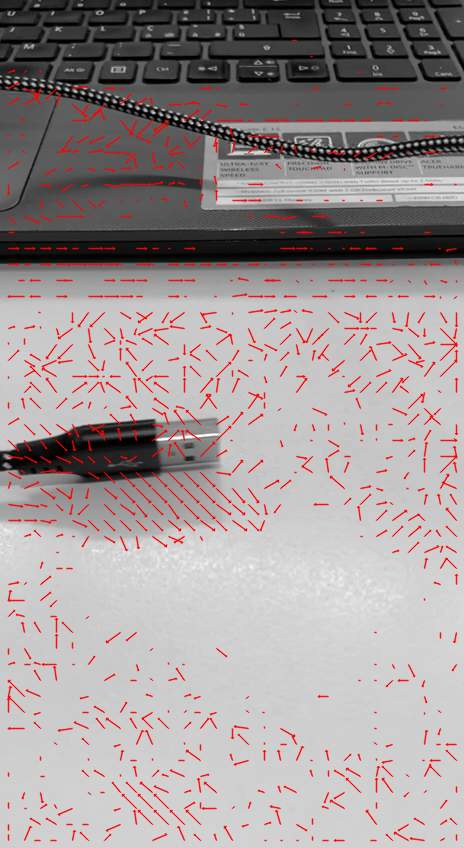
\includegraphics[keepaspectratio, width=.55\linewidth]{images/bbme-1-res.png}
            \subcaption{Needle diagram}
            \label{fig:bbme-1-res}
		\end{minipage}
		% \begin{minipage}{.3\textwidth}
        %     \centering
        %     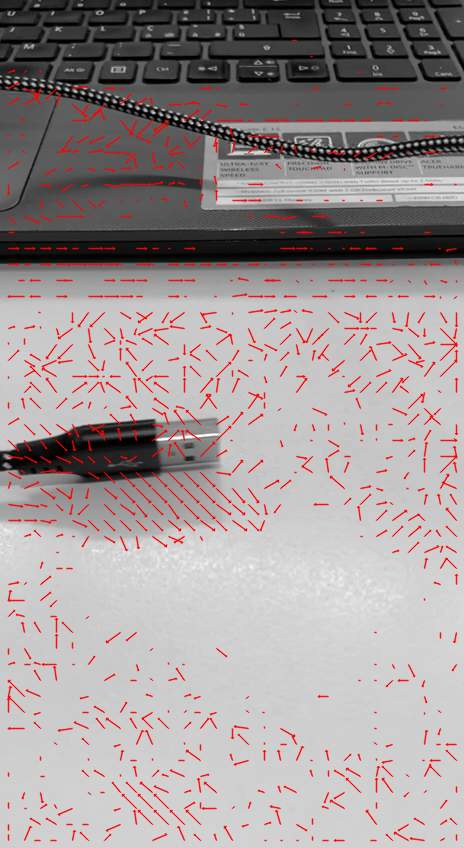
\includegraphics[keepaspectratio, width=.8\linewidth]{images/bbme-1-res.png}
        %     \subcaption{Hierarchical version}
        %     \label{fig:bbme-h1-res}
		% \end{minipage}
        \label{fig:bbme-1}
        \caption{Motion field result of our TSS implementation}
	\end{figure}
\end{frame}

\begin{frame}{2D Log search}
	\begin{figure}
		\begin{minipage}{.45\textwidth}
            \centering
            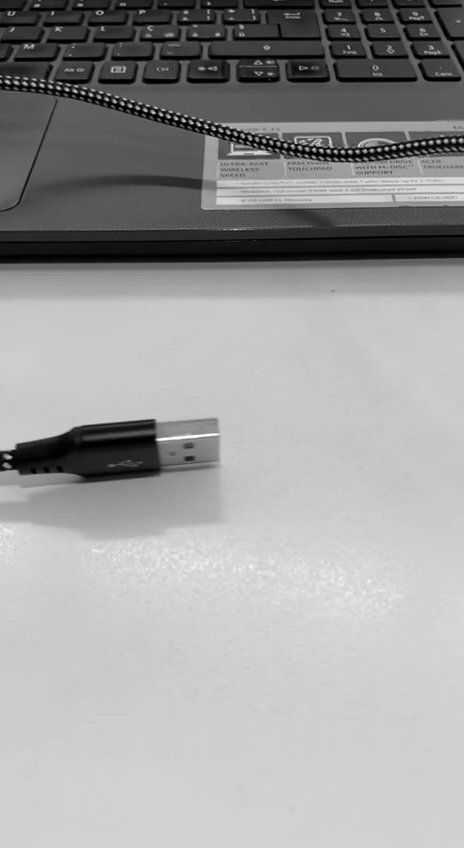
\includegraphics[keepaspectratio, width=.55\linewidth]{images/bbme-im.png}
            \subcaption{Target frame}
            \label{fig:bbme-2-im}
		\end{minipage}
		\begin{minipage}{.45\textwidth}
            \centering
            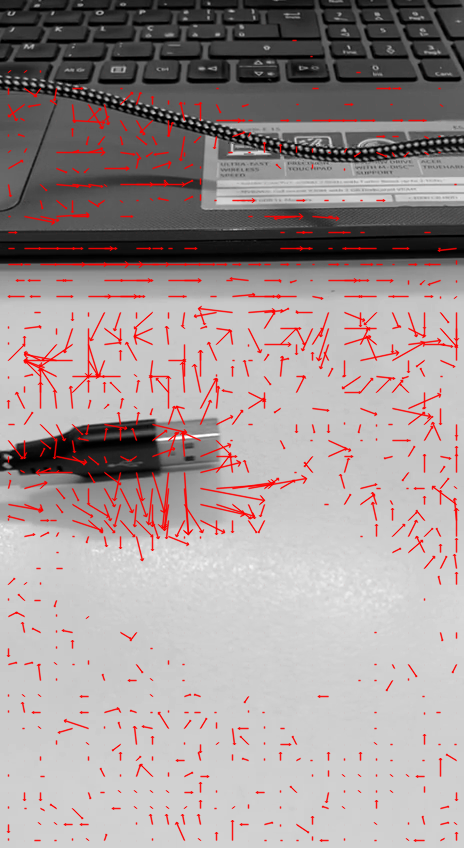
\includegraphics[keepaspectratio, width=.55\linewidth]{images/bbme-2-res.png}
            \subcaption{Needle diagram}
            \label{fig:bbme-2-res}
		\end{minipage}
        \label{fig:bbme-2}
        \caption{Motion field result of our TDLS implementation}
	\end{figure}
\end{frame}

\subsubsection*{Diamond search BBME}
\begin{frame}{Diamond search}
	BBME algorithm presented in Zhu and Ma, 2000. Better performances thant classic algorithms (TSS) and comparable to latest ones (NTSS), yet more efficient in computation.
    \bigskip
    
    It uses two different search patterns, both of which are diamond-shaped:
    \begin{itemize}
        \item large diamond search pattern (LDSP)
        \item small diamond search pattern (SDSP)
    \end{itemize}
    \begin{figure}
        \centering
        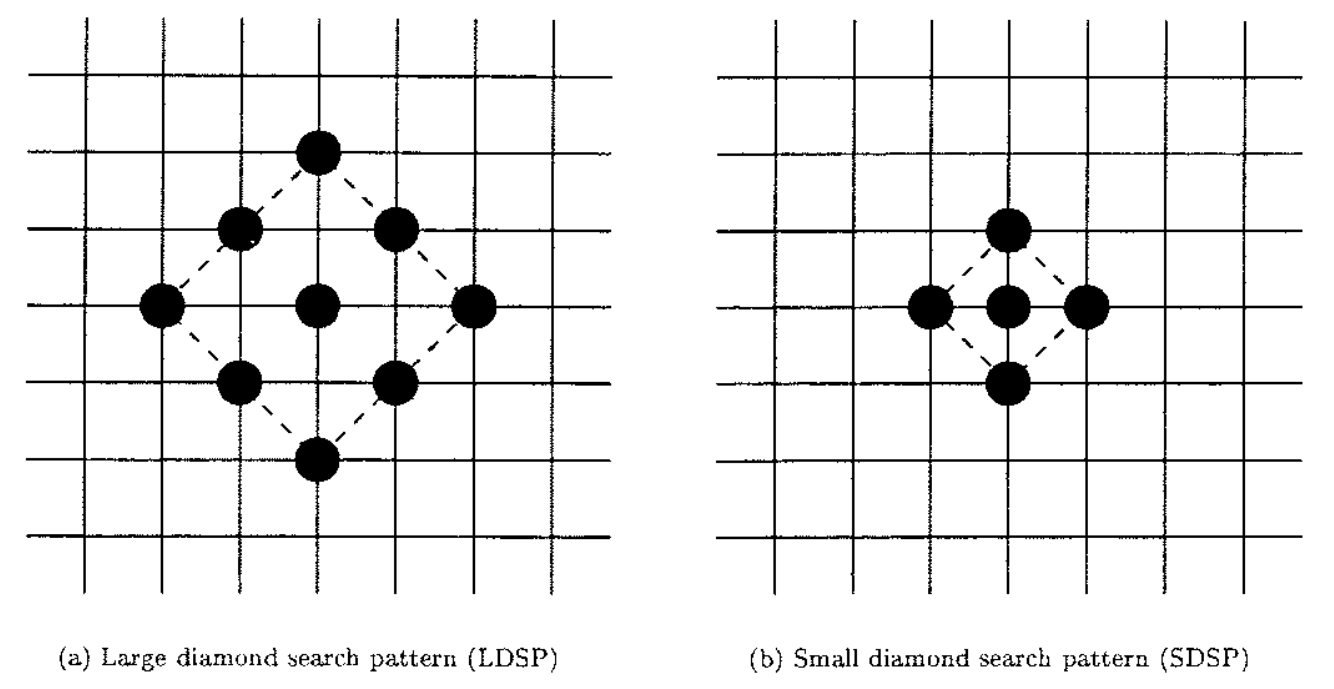
\includegraphics[keepaspectratio,width=.5\linewidth]{images/ds-search-patterns.png}
        \caption{The shape of LDSP and SDSP}
    \end{figure}
\end{frame}

\begin{frame}{DS algorithm}
    \begin{block}{Diamond search procedure}
        For each block:
        \begin{enumerate}
            \item place LDSP in the center of the block and compute DFD for all of the 9 displacements;
            \begin{itemize}
                \item if the minimum DFD is in the center position, then go to 3
                \item else, go to 2
            \end{itemize}
            \item reposition LDSP in the minimum DFD of the previous operation and recompute DFD;
            \begin{itemize}
                \item if the minimum DFD is in the center position, then go to 3
                \item else, repeat 
            \end{itemize}
            \item place SDSP, compute DFD and return coordinates of the minum DFD block as motion vector
        \end{enumerate}
    \end{block}
\end{frame}

\begin{frame}{DS algorithm visualized}
    \begin{figure}
        \centering
        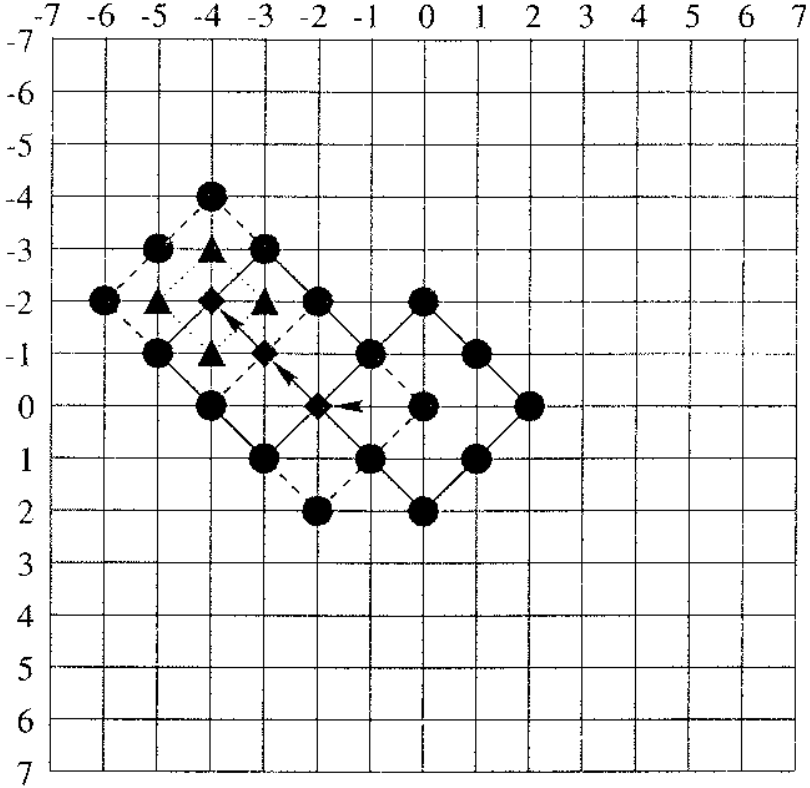
\includegraphics[keepaspectratio,width=.45\linewidth]{images/ds-exe.png}
        \caption{Example of a full execution cycle of diamond search}
    \end{figure}    
\end{frame}

\begin{frame}{DS results}
	\begin{figure}[H]
		\begin{minipage}[b]{0.45\textwidth}
            \centering
            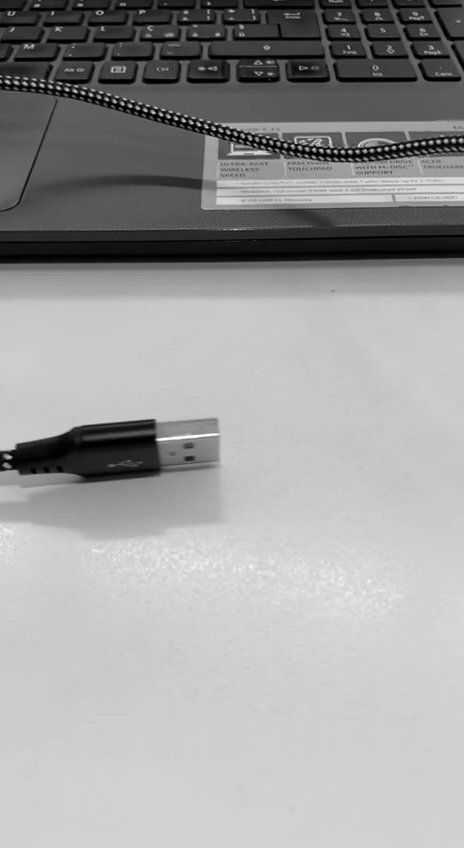
\includegraphics[keepaspectratio, width=.55\linewidth]{images/bbme-im.png}
            \label{fig:bbme-3-im}
            \subcaption{Target frame}
		\end{minipage}%
		\begin{minipage}[b]{0.45\textwidth}
            \centering
            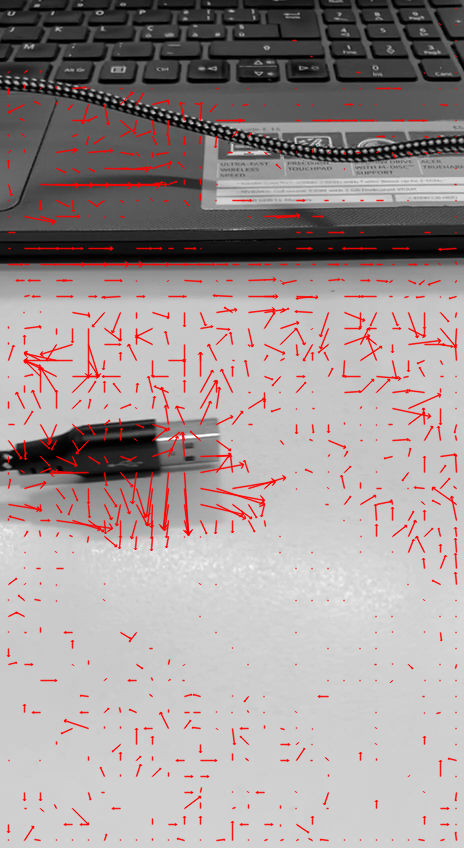
\includegraphics[keepaspectratio, width=.55\linewidth]{images/bbme-3-res.png}
            \label{fig:bbme-3-res}
            \subcaption{Needle diagram}
		\end{minipage}
        \label{fig:bbme-3}
        \caption{Motion field result of our DS implementation}
	\end{figure}
\end{frame}

\subsection{Global motion estimation}
\begin{frame}{The affine model}
    It features a six parameters vector \(a = [a_0, a_1, a_2, b_0, b_1, b_2]^T\)
    \bigskip

    The parameter matrix looks like this 
    \begin{equation*}
        [A(x)] = 
        \begin{bmatrix}
            1 & x & y & 0 & 0 & 0 \\
            0 & 0 & 0 & 1 & x & y
        \end{bmatrix}
    \end{equation*}
\end{frame}

\begin{frame}{Robust}
    
\end{frame}


\section{Evaluation}
\subsection{Qualitative: motion compensation}
\begin{frame}{Compensation}

\end{frame}
\subsection{Quantitative: PSNR}

\section{Conclusions}

\begin{frame}
    \begin{center}
        {\Huge\calligra Thanks!}
    \end{center}
\end{frame}

\end{document}